\section{Introduction}
\label{sec-introduction}

As personal wireless devices proliferate over the last decade, more and more
\wifi{} Access Points (APs) are deployed to meet the increasing demand for
pervasive network access. By the end of 2014, 451 million households worldwide
(65\% of total the 690 million) use wireless routers to extend their network access
beyond the fix-line broadband, and the penetration is expected to
grow to 80\% by 2018~\cite{survey}.

However, due to factors such as blockage or fading of wireless signals, home AP
usually does not provide equally satisfying \wifi{} coverage at all places
within the house. Instead, it is likely that the user receives better \wifi{}
signals from neighbors' APs at certain spots. For instance, consider Alice and
Bob who live in neighbor apartments, as shown in Figure~\ref{fig:motivation},
each of them receives a stronger \wifi{} signal from the other's home AP than
their own at certain places within their apartments, revealing a
\textit{reciprocal} \wifi{} sharing opportunity where both parties can improve
their \wifi{} performance by allowing each other to access their own private
networks.

Compared to traditional community networks such as FON~\cite{fon} or
OpenWireless~\cite{openwireless}, such reciprocal sharing opportunity has
several unique properties that make it interesting to explore. First, such
opportunity is usually \textit{immediate} between two physically colocated
parties, such as two neighbors. This helps relief the concerns or trust issues
of sharing network to random strangers in traditional community networks, and
also makes it easy to coordinate the sharing. Second, bonding to physical
colation relationship makes the opportunity \textit{stable} over time, making it
possible to enable fair sharing asynchronously over longer period of time.

\begin{figure}[t]
  \centering
  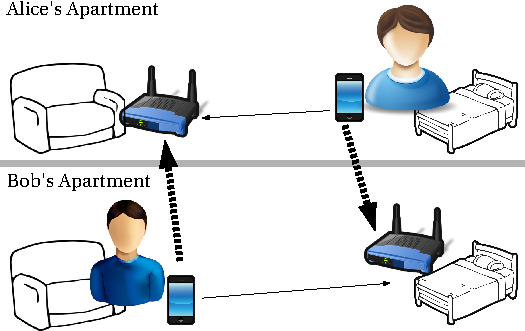
\includegraphics[width=\columnwidth]{./figures/motivation.pdf}
  \caption{\textbf{An Example of Reciprocal \wifi{} Sharing.} Solid arrows
    represent existing associations with weak signal. Dashed arrows indicate
  potentially better associations with stronger \wifi{} signal.}
  \label{fig:motivation}
\end{figure}

Nevertheless, there are several challenges in fulfilling the vision of
reciprocal \wifi{} sharing shown in Figure~\ref{fig:motivation}. First, although
the motivation example is inspired by the authors' own experience, it is not
clear how often such opportunity exists for broader range of users in real life
scenarios. Second, suppose the sharing opportunity does exist and is detected,
there is no systematic solutions to enable the \wifi{} sharing without
compromising the security and privacy of user's home network. Finally, after the
\wifi{} sharing is established, it is challenging to ensure that the
relationship remains reciprocal for both parties.

To address these challenges, we first present extensive analysis of the
\PhoneLab{} \wifi{} dataset which contains \num{21192417} scan results from 254
smartphones over 5 months (Section~\ref{sec:investigation}). The results show
that such reciprocal \wifi{} sharing opportunities does exists even in a sparse
dataset. Inspired by the results, we present the design of \wisefi{}
(Section~\ref{sec:design}), a system that detects such reciprocal \wifi{}
sharing opportunities using smartphones, enables \wifi{} sharing on APs with or
without guest network support, and ensures the sharing remain reciprocal.
Finally, we discuss some open challenges in implementing such a system and point
directions for future works (Section~\ref{sec:challenges}).
